Para representar ondas matemáticamente se utilizan las funciones $\sin(x)$ y $\cos(x)$.

\begin{tikzpicture}
  \begin{axis}[
    xmin=0,xmax=2.2*pi,
    ymin=-1.2,ymax=1.2,
    axis lines=middle,
    xtick={0},
    xtick={pi/2,pi,3*pi/2,2*pi},
    xticklabels={
      $\dfrac{\pi}{2}$,
      $\pi$,
      $\dfrac{3}{2}\pi$,
      $2\pi$
    },
    xticklabel style={anchor=south west},
    ytick={-1,1},yticklabels={$-1$,$1$}
    % ylabel=Desplazamiento
    ]

    % Funcion senoidal
    \addplot[color=blue,samples=100,domain=0:2*pi,thick]{sin(deg(x))}
    node[right,pos=0.9]{$\sin(x)$};

    % Funcion cosenoidal
    \addplot[color=red,samples=100,domain=0:2*pi,thick]{cos(deg(x))}
    node[right,pos=0.9]{$\cos(x)$};
  \end{axis}
\end{tikzpicture}

Estas funciones se pueden modificar mediante ciertos valores. La forma matemáticamente de esto es la siguiente:

\begin{listequbox}
  {f(x) = A\sin(fx-\phi)}{ondasencilla}{Función sencilla de onda}
\end{listequbox}
